\documentclass[a4paper,11pt]{article}
\usepackage{ls}
\usepackage[utf8]{inputenc}
\usepackage[main=russian,ngerman]{babel}

\author{Hans-Gert Gräbe}
\title{Отчет о семинаре 12 января 2021 г.}
\date{30.01.2021}

\begin{document}
\maketitle

\section{О назначении семинара}
Термин система играет важную роль в информатике, когда речь идет о системе
базах данных, системы программного обеспечения, системы компютерной техники,
системы учета, системы доступа и другие. В общем, множество экспертов
определяет информатику как «наука \emph{систематического} представления,
хранения, обработки и передачи информации, особенно автоматической обработкой
с помощью вычислительных машин» (немецкая википедия). Также некоторые
актуальные профессии, такие как \emph{системный архитект} высоко ценятся
ИТ-пользователями.

Однако значение термина «система» выходит далеко за пределы области
информатики -- это фундамент всех инженерных наук и как \emph{системная
  инженерия} в стандарте ISO/IEC/IEEE-15288 «Systems and Software Engineering»
является предметом интернациональных процессов нормирования и
стандартизации. Термин системы также играет центальную роль при описании
сложных природных и культурных процессов -- например, в термине
\emph{экосистемы}.

С \emph{семантическими сетями} на первый план выходит анализ значений цифровых
артефактов, которые в конце концов являются языковыми артефактами и поэтому
также напрямую связаны с умело развернутой \emph{концепции системы}, лежащей в
основе каждого понимания конкретной системы.

Наконец, модное слово \emph{устойчивость} используется для описания сложных
процессов социального согласования, связанные с многочисленными проблемами
информации и оценок. Здесь умение описательного разграничения, развития и
управления так называемых систем на различных уровнях управления, пространства
и времени имеет большое значение.

В зимнем семестре 2019/20 мы уже имели дело с этим спектром \emph{системных
  подходов} (во множественном числе), изучали широкий спектр соответствующих
концепций из разных областей науки, и сравнили их в последней части семинара с
подходом к развитию технических систем в контексте ТРИЗ. Эти исследования мы
постараемся углублять в текущем исследовательском семинаре.

\begin{quote}
  \textbf{Цель семинара} -- лучше понять различные концепции законов,
  закономерностей, тенденции и паттерны развития технических и общих систем,
  предложенные и разработанные в контексте ТРИЗ.
\end{quote}

Подробнее о семинаре (на немецком языке) в нашем github репозитории
\begin{center}
  \url{https://github.com/wumm-project/Leipzig-Seminar}.
\end{center}

Темой семинара, о котором тут идет речь, была \emph{эволюция технических и
  общих систем у М.С. Рубина}. Отправной точкой и основой семинара и
обсуждения служил \cite{Rubin2019}.

Этот текст состоит из трех частей,
\begin{itemize}[noitemsep]
\item мои заметки к семинару,
\item комментируемый чат семинара,
\item раздаточный материал, подготовленный Иммануэлем Токе.
\end{itemize}

\section{Заметки}

На протяжении многих лет М.С. Рубин занимается вопросом, как законы,
тенденции и линии развития технических и общих систем можно соединить в единый
концепт. См. например сайт \url{http://www.temm.ru}, на котором собраны тексты
\textbf{теории эволюции материи и моделей}, в которых исследуются связи между
материальными явлениями и их формами описания. Представлены тексты Михаила
Рубина и Юлия Мурашковского, причем Рубин больше сосредоточится на вопросах
связи между материалными и нематериальными системами, Мурашковский более на
социокультурных системах. 

В \cite{Rubin2019} сравниваются не только варианты законов развития
технических систем в различных школах ТРИЗ, но также (там же, рис. 3)
представлена попытка связать эти законы с различными инструментами ТРИЗ и в
конечном итоге отметить закрепление законов в алгоритме АРИЗ.

Рубин различает законы и тренды, последние (тренды) как «основная тенденция
изменения чего-либо». Различие «между законом и тенденциями» является
«очевидным и принципиальным». Это различение существенное, потому что,
например, «тенденции моды» или «тенденции погоды» не имеют характера законов
(как «необходимое, существенное, повторяющееся»).  Концепция закона глубже в
своих требованиях к обоснованию, но действие законов \emph{выявляется} не
только в \emph{инвариантах} (например, в законе сохранения энергии или в
утвеждении Галилея о том, что лист и камень падают с одинаковой скоростью), но
также может выявляться  как тренд (в смысле текущего равновесия). Дальше это в 
семинаре не обсуждалось. 

По словам Рубина, разработка технических систем (ТС) может происходить на трех
уровнях, как изменение (реальной) системы (формы исполнения), как изменение
модели (форма описания в виде белого ящика со ссылкой на ту же систему
реального мира) и как изменение принципа действия (изменение реализации с той
же спецификацией).

Таким образом, развитие системы всегда связано с ее преобразованием. Поэтому
преобразования (от \emph{системы с проблемой} к \emph{системе без проблем}, от
«системы, как она есть» к «системе, как она должна быть») являются основой
ТРИЗ, и также понятно, что ТРИЗ по сути \emph{реализует} идею развития, так
что его \emph{теоретическое обоснование} существенно для системы теории ТРИЗ.

Дальше обсуждались понятия \emph{филогенез} и \emph{онтогенез} ТС (даже если
Рубин эти понятия всегда сопровождает прилагательным «системный»). Это
разделение в долгосрочные и краткосрочные перспективы развития, которое должно
улавливаться в этой заимствованной из биологии терминологии, вызывало большое
недоразумение, даже если мы и раньше столкнулись с отчужденным использованием
терминов, заимствованных из биологии, в контексте «технической
экосистемы». Кен Клеманн отметил, что эти понятия были введены Дарвином и
особенно Эрнстом
Геккелом\footnote{\url{https://de.wikipedia.org/wiki/Biogenetische_Grundregel}}
во второй половине XIX века, чтобы установить отношения между племенным и
индивидуальным развитием. Однако в основе (биологической) концепции филогенеза
лежит воспроизведение внутри вида и, таким образом, четкое, наблюдаемое в
реальном мире соотношение воспроизводства.  Эпигенетические факторы окружающей
среды в значительной степени игнорировались, их значение становится все более
очевидным за последние 50 лет.  (Биологические) линии эволюции на более
высоких уровнях агрегации (род, семья, отряд, класс, племя) тогда обоснованы
только ещё на умственных агрегатах.  Ответ на вопрос о том, как Рубин
переносит эти конструкции в «мир технических систем» остался непонятным,
поскольку репродуктивные отношения здесь -- по сравнению с биологией --
совершенно другие. Особенно утверждения «Законы связаны с филогенезом и
являются инструментами для трансформации ТС в онтогенезе» и в результате
заключение «Выявление существования законов развития ТС требует наличие и
выявление филогенетических процессов в ТС» оставалось непонятным.

Наконец, обсуждалось, что концепция ТС Альтшуллера основана на концепции
полезной функции (ГФ), в то время как более крупные системы, как правило,
являются \emph{мультифункциональными}, в которых разделение системных функций
на \emph{одну} доминирующую главную функция и \emph{несколько} дополнительных
или вспомогательных функций в общем трудновато и отчасти не возможно.

\section{Прокомментированный чат}

\subsection*{Ещё раз онтогенез и филогенез}

Слайд 11: Если ТРИЗ означает трансформацию (в одной из коробок), то в картине
показан сценарий трансформации трансформаций.

\begin{center}
  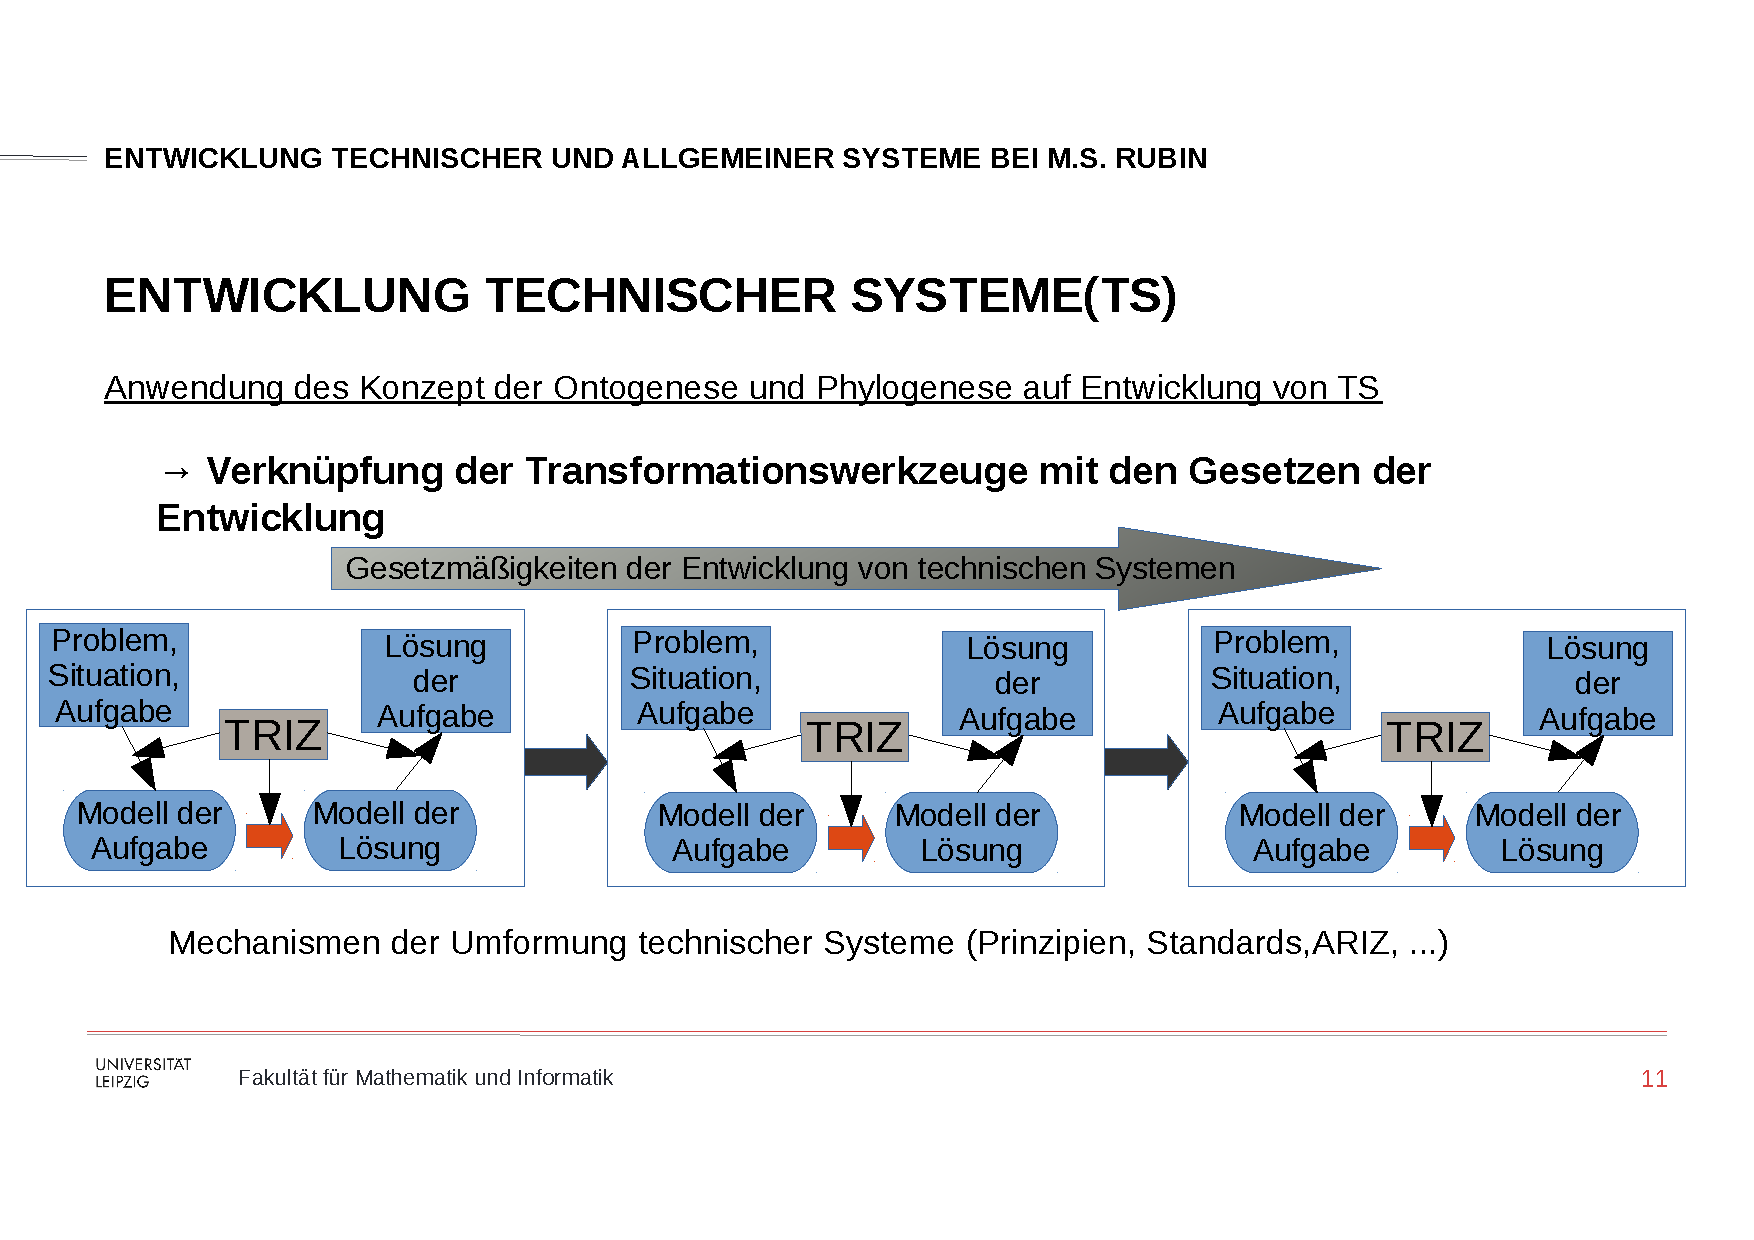
\includegraphics[width=.7\textwidth]{Folie11.pdf}
\end{center}

Согласно рисунку \emph{онтогенез} -- это решение проблемы путем преобразования
одного ТС в одном из ящиков и \emph{филогенез} -- развитие самого процесса
решения путем применения системного преобразования, т.е. путем преобразования
самого процесса преобразования.

\subsection*{Различные сборники законов}

Рубин называет 9 законов, в \cite{Altschuller1979} упоминается только
8. Откуда разница? 

\emph{Закон динамизации TS} (больше?) не упоминается в \cite{Altschuller1979}
и \cite{Altschuller1980}.

\subsection*{Откуда взялась S-образная кривая?}

За S-образной кривой стоит математическая модель \emph{логистической
  функции}\footnote{\url{https://de.wikipedia.org/wiki/Logistische_Funktion}}
-- это решение простой экспоненциальной зависимости развития с эффектом
насыщения. 

В \cite{Altschuller1979} и \cite{Altschuller1980} такая кривая называется
\emph{линией жизни}, в \cite{Altschuller1979} сначала в разделе 7.1
развивается «линия жизни», а затем в разделе 7.3 законы, а в
\cite{Altschuller1980} наоборот.

Для Рубина это скорее паттерн из нескольких возможных, а также больше
(необязательный) образ мышления, а не эмпирически подтвержденный факт. 
Тем более что единицы измерения на ординате остаются туманными (Рубин, следуя
Альтшуллеру: «Основные характеристики, такие как емкость, производительность,
скорость и т.д.»).

Альтшуллер также использует вертикальные разрезы, чтобы спроецировать в эту
лишь качаственную диаграмму фазовую модель развития («детство», «зрелость»,
«старость», а затем альтернативно «застой» или «деградация»).

\subsection*{МАТХЭМ}

Слайд 17 и 18 (Мифы об основах разработки технических систем)

Термин поля в ТРИЗ -- смутное понятие.

В дуализме волны и частицы физики действия распространяются волнообразно, но
опосредованы частицами. Например, глюоны образуют обменные частицы сильного
взаимодействие. Похожим образом «фонон является элементарным возбуждением
(квант) упругого поля» (немецкая википедия), т.е. термин «поле» уже
используется в физике инфляционно, когда дело доходит до моделирования
причинно-следственных связей. Это продолжается в ТРИЗ, если необходимо
концептуализировать принципы инженерно-технического решения (например, А стоит
для «акустического поля» и, следовательно, для этого самого «упругое поле»
физики).

Сегодня это часто дополняется I (информация) и B (биология), например
\cite{Belski2016}.

Однако теория ТРИЗ также имеет дело с использованием конкретных научных
эффектов. Поэтому понятие поля тоже стоит за связь между научным знанием и
инженерными техническими приложениями.

\section{Развитие технических и общих систем у М.С. Рубина}

\begin{center}
  Раздаточный материал Иммануэля Тока, 10 января 2021 г.
\end{center}

\subsection{Циклы системной науки}
«Стремительное развитие окружающего нас мира делает насущной необходимость
разработки всеобщих и прикладных теорий, на основе которых возникающие
проблемы в различных областях могут быть эффективно решены.» \cite{Rubin2002} 

Читая эту цитату, трудно не вспомнить таких классических эрудитов, как
Леонардо да Винчи или Готфрид Вильгельм Лейбниц. Является ли упрощенная
доступность к все более широкому и глубокому цифровому хранилищу знаний и
возможности доступа к учреждениям науки для все более широкого населения
причиной того, что тип \emph{универсального ученого} станет разпространенным
явлением? Требует ли это новые методы для организации этого знания --
циклическое «перегружение» (в смысле устаревания предыдущих методов), что
делает сокращение и структурирование необходимым для того, чтобы хотя иметь
чувство, что обзор не потерян -- или сама материя открывает вид на
систематические связи? 

В то же время, если смотреть, в частности, на научно-популярные cредства
массовой информации, кажется, что существует тенденция сосредоточиться на
особо (экономически) привлекательных темах. Так сейчас разпространенное
явление изучать неврологию, астрономию, физику частицу или метафизику. Хотя
оригинальная экспертиза на первый взгляд имеет мало общего с обсуждаемыми
темами, выявляются паттерны, которые приведут к инфрадисциплинарному
исследованию специфики и возможных дженериков. Несмотря на то что в публичных
обсуждениях регулярно путают научно-популярные аналогии с специальными
терминами предмета -- этот аспект межпарадигматического структурного
творчества является знаком «системного включения», особенно в областях
полей научных исследований -- подумать только о развитии нейронных сетей.

Рубин изначально проводит грубое различие между материальными и
нематериальными системами. При этом категория материальных систем
разпространяется от неорганических и органических (физически-химических),
живых (биофизико-химических) до социальных и социально-технических систем. Для
него все эти системы имеют «единые законы развития» \cite{Rubin2002}.
Нематериальные системы связаны с «появлением человека, разума и цивилизации»
\cite{Rubin2006} и вместе с ним «таких систем, как наука, искусство, религия,
технологии, язык и многих других» \cite{Rubin2006}. Остается неясным, следует
понимать ли это как вид «метафизической системы» или описывается, как люди
ведут себя в онтологической системе. Он собирает нематериальные системы под
понятием \emph{культуры} и одновременно указывает на проблему нормативного
характера тех законов, которые обычно называют законами природы.  Он приводит
примеры как «мировоззрение как поле битвы теорий и людей», ревизия теории
флогистона и различные примеры «структурной индукция» по законам как
«необходимые, существенные, устойчивые, повторяющиеся отношения между
явлениями в природе и обществе». Понятие природы здесь более вероятно надо
понять в переносном смысле, как надсистему и общепризнанные рамки действий --
как например, древние календари, традиции или июридические рамки.

Связь между инструментами трансформации и законами развития систем является
центральным аспектом его методологии. Сначала это кажется тривиальным, но
понимается как важная характеристика системной науки \cite{Kleemann2020} --
что это особенно важно для этапов преобразования модели, но не обязательно
переносится на методы реализации, подробно обсуждалось на семинаре. В то же
время это открывает неоднозначность термина \emph{развитие}, и возникает
вопрос, насколько единство системы и метода как единство теории и практики
действительно имеет значение, если учесть интерсубъективную семантику
терминов.

\subsection{Аналогизмы инфрадисциплинарной систематики}

«То, что физики называют законом, математики называют гипотезой.» (Скотт
Ааронсон)

Возможно, просто очевидно, почему Рубин использует биологические термины,
чтобы описать и категоризировать паттерн в развитии систем средствами
онтогенеза и филогенеза. Биология -- в конце концов --  является исторически
ранной междисциплинарной системной наукой, которая не позже чем со времен
Менделя и Дарвина занимается описанием характеристик и структурного 
развития.

Однако возникает вопрос, в какой степени термины одной дисциплины
принципиально переносимы к другим дисциплинам, или в их применении в чужих
контекстах выражается терминологическое различие в том смысле, что применение
терминов в чужой дисциплине является только первым шагом приближения к новой
терминологической информации в другой дисциплине, а приближение 
может быть только асимптотическим. С аналогиями игра быстро набирает
обороты. Мамонт может приравняться с конной повозкой, а слон с двигателем
внутреннего сгорания. Ортологические отношения, вытекающие из
филогенетических информаций, могут быть перенесены на элементы машины
автомобиля.  Эта аналогия терминов приводит к структурной
эквивалентности и, следовательно, к проблеме. Структурная
эквивалентность применима только в пределах предметных границ. Для трансфера
знаний за эти границы каждый раз требуется усилие перевода.  Усилие перевода
переходит в слияние хотя бы тогда, когда необходимы юридически значимые
определения, чтобы сделать запланированные системы пригодными для
повседневного использования. Тогда изчесают субъективные границы первого
порядка и, следовательно, появляется единство социотехнических систем и их
методологии в долгосрочной перспективе. 

Как известно, закон слепой, и, возможно, помогает только поле напряжения
эвристики, как это отражено в теории систем Лумана.  Насколько грамматики
людей, коммуникативные выводы которых не отображаются друг на друга биективным
способом, рационализируют иррациональные процессы в виде конформных с их
ожиданиями институты, настолько эти же люди сформируют свой собственный
«объективный» закон второго порядка, которому они обьязаны подчиняться, чтобы
понять друг друга. Соглашаясь на общую формулировку и подтвердив
приблизительное отображение частных семантик вместо поиска противоречий в
предположительно недостаточной точности, практика этих соглашений открывает
пространство для разнообразия индивидуальных нюансов понятий, но и путь к
общему действию и тем самым к новому опыту, новому переосмыслению
индивидуальных нюансов понятий в зависимости от контекста процесса, включая
обратную связь динамического социального контекста. 

В этом смысле значение термина \emph{совпадает} с его употреблением.

\begin{thebibliography}{yyy}
\bibitem{Altschuller1979} Genrich S. Altshuller (1979).  Творчество как
  точная наука.  Немецкий перевод 1983: \emph{Erfinden -- (k)ein Problem}.
\bibitem{Altschuller1980} Genrich S. Altshuller, Alexander B. Seljutsky
  (1980). Крылья для Икара. Немецкий перевод 1983: \emph{Flügel für Ikarus}.
\bibitem{Belski2016} Iouri Belski, Pavel Livotov, Oliver Mayer (2016). Eight
  Fields of MATCEMIB Help Students to Generate More Ideas. Procedia CIRP
  39:85-90.  DOI \texttt{10.1016/j.procir.2016.01.170}
\bibitem{Kleemann2020} Ken P. Kleemann (2020). Dialektik der kreativen
  Innovation (Диалектика творческих инноваций).  In: Erfinderschulen, TRIZ und
  Dialektik. Rainer Thiel zum 90. Geburtstag.  Rohrbacher Manuskripte, Heft
  20. ISBN 9783751983228.
\bibitem{Rubin2002} Michail S. Rubin (2002).  О теории развития материальных
  систем (ТРМС). \\ \url{http://www.temm.ru/ru/section.php?docId=3878}.
\bibitem{Rubin2006} Michail S. Rubin (2006). Принцип захвата и многообразия в
  развитии систем.\\ \url{http://www.temm.ru/ru/section.php?docId=3433#2}.
\bibitem{Rubin2019} Michail S. Rubin (2019).  О связи комплекса законов
  развития систем с ЗРТС.  Рукопись, 06.11.2019. Немецкий перевод 2020.
\end{thebibliography}


\end{document}
